\documentclass[11pt,a4paper]{article}
\usepackage[margin=2.4cm]{geometry}
\usepackage{graphicx}
\usepackage{booktabs}
\usepackage[hidelinks]{hyperref}
\usepackage{caption}
\captionsetup{font=small,labelfont=bf}

\title{\textbf{PD-RobustBench -- Supplementary Material}\\
\large Corruption-Robustness and Explainability Evaluation for
PD Detection from Hand-Drawn Images}
\author{Torik, Abedini, Peyvandi}
\date{}

\begin{document}
\maketitle

\section*{S1. Validation-selected decision thresholds}
Per-model decision thresholds chosen on the validation split to maximize
balanced accuracy (Section~3.2 of the main text). The same threshold is
applied to the clean and to every corrupted condition of that model.

\begin{table}[h]
\centering\small
\begin{tabular}{llc}
\toprule
Dataset & Model & Threshold \\
\midrule
HandPD--meander & ResNet50 & 0.90 \\
HandPD--meander & VGG16 & 0.60 \\
HandPD--meander & EffNet-B0 & 0.75 \\
HandPD--meander & MobileNetV3 & 0.95 \\
HandPD--spiral & ResNet50 & 0.95 \\
HandPD--spiral & VGG16 & 0.45 \\
HandPD--spiral & EffNet-B0 & 0.50 \\
HandPD--spiral & MobileNetV3 & 0.45 \\
PDRAW--spiral & ResNet50 & 0.50 \\
PDRAW--spiral & VGG16 & 0.50 \\
PDRAW--spiral & EffNet-B0 & 0.50 \\
PDRAW--spiral & MobileNetV3 & 0.50 \\
PDRAW--wave & ResNet50 & 0.55 \\
PDRAW--wave & VGG16 & 0.45 \\
PDRAW--wave & EffNet-B0 & 0.35 \\
PDRAW--wave & MobileNetV3 & 0.65 \\

\bottomrule
\end{tabular}
\caption{Validation-selected decision thresholds.}
\end{table}

\section*{S2. Bootstrap confidence intervals for clean metrics}
Bootstrap 95\% intervals (2{,}000 resamples of per-image predictions, seed 42)
for clean accuracy and ROC-AUC. Intervals are wide because test sets contain
30 (PDRAW) or 108 (HandPD) images; see the Uncertainty paragraph in the
main text.

\begin{table}[h]
\centering\small
\begin{tabular}{lllc}
\toprule
Dataset & Model & Metric & Point estimate [95\% CI] \\
\midrule
HandPD--meander & EffNet-B0 & Accuracy & 0.833 & [0.759, 0.898] \\
HandPD--meander & EffNet-B0 & ROC-AUC & 0.823 & [0.669, 0.946] \\
HandPD--meander & MobileNetV3 & Accuracy & 0.759 & [0.676, 0.843] \\
HandPD--meander & MobileNetV3 & ROC-AUC & 0.835 & [0.695, 0.956] \\
HandPD--meander & ResNet50 & Accuracy & 0.852 & [0.787, 0.917] \\
HandPD--meander & ResNet50 & ROC-AUC & 0.857 & [0.741, 0.951] \\
HandPD--meander & VGG16 & Accuracy & 0.898 & [0.833, 0.954] \\
HandPD--meander & VGG16 & ROC-AUC & 0.857 & [0.740, 0.950] \\
HandPD--spiral & EffNet-B0 & Accuracy & 0.843 & [0.768, 0.907] \\
HandPD--spiral & EffNet-B0 & ROC-AUC & 0.978 & [0.950, 0.996] \\
HandPD--spiral & MobileNetV3 & Accuracy & 0.870 & [0.806, 0.926] \\
HandPD--spiral & MobileNetV3 & ROC-AUC & 0.944 & [0.895, 0.982] \\
HandPD--spiral & ResNet50 & Accuracy & 0.880 & [0.815, 0.935] \\
HandPD--spiral & ResNet50 & ROC-AUC & 0.972 & [0.938, 0.994] \\
HandPD--spiral & VGG16 & Accuracy & 0.889 & [0.824, 0.944] \\
HandPD--spiral & VGG16 & ROC-AUC & 0.916 & [0.837, 0.976] \\
PDRAW--spiral & EffNet-B0 & Accuracy & 0.767 & [0.600, 0.900] \\
PDRAW--spiral & EffNet-B0 & ROC-AUC & 0.867 & [0.727, 0.978] \\
PDRAW--spiral & MobileNetV3 & Accuracy & 0.800 & [0.667, 0.933] \\
PDRAW--spiral & MobileNetV3 & ROC-AUC & 0.924 & [0.818, 0.996] \\
PDRAW--spiral & ResNet50 & Accuracy & 0.733 & [0.567, 0.900] \\
PDRAW--spiral & ResNet50 & ROC-AUC & 0.924 & [0.817, 0.996] \\
PDRAW--spiral & VGG16 & Accuracy & 0.733 & [0.567, 0.868] \\
PDRAW--spiral & VGG16 & ROC-AUC & 0.818 & [0.642, 0.955] \\
PDRAW--wave & EffNet-B0 & Accuracy & 0.733 & [0.567, 0.900] \\
PDRAW--wave & EffNet-B0 & ROC-AUC & 0.938 & [0.826, 1.000] \\
PDRAW--wave & MobileNetV3 & Accuracy & 0.900 & [0.767, 1.000] \\
PDRAW--wave & MobileNetV3 & ROC-AUC & 0.929 & [0.804, 1.000] \\
PDRAW--wave & ResNet50 & Accuracy & 0.800 & [0.633, 0.933] \\
PDRAW--wave & ResNet50 & ROC-AUC & 0.907 & [0.778, 0.991] \\
PDRAW--wave & VGG16 & Accuracy & 0.900 & [0.800, 1.000] \\
PDRAW--wave & VGG16 & ROC-AUC & 0.898 & [0.742, 1.000] \\

\bottomrule
\end{tabular}
\caption{Clean test metrics with bootstrap 95\% confidence intervals.}
\end{table}

\section*{S3. PRS weight-sensitivity analysis}
PRS recomputed under the main weighting $(0.50, 0.30, 0.20)$, a
performance-only weighting $(0.70, 0.30, 0.00)$, and an equal weighting
$(1/3, 1/3, 1/3)$. The model ranking per image type is identical under all
three weightings (Spearman $\rho = 1.0$); the performance-only weighting
yields a clipped score of 100 for EfficientNet-B0 on PDRAW--wave because its
net degradation over the severity range is non-positive.

\begin{table}[h]
\centering\small
\begin{tabular}{llccc}
\toprule
Dataset & Model & $w=(.5,.3,.2)$ & $(.7,.3,0)$ & $(1/3,\,1/3,\,1/3)$ \\
\midrule
HandPD--meander & EffNet-B0 & 82.4 & 84.4 & 80.7 \\
HandPD--meander & MobileNetV3 & 84.5 & 86.2 & 83.1 \\
HandPD--meander & ResNet50 & 92.5 & 96.3 & 89.8 \\
HandPD--meander & VGG16 & 88.9 & 90.8 & 87.5 \\
HandPD--spiral & EffNet-B0 & 87.9 & 92.0 & 85.3 \\
HandPD--spiral & MobileNetV3 & 94.9 & 97.1 & 93.5 \\
HandPD--spiral & ResNet50 & 90.7 & 94.1 & 88.6 \\
HandPD--spiral & VGG16 & 94.3 & 98.0 & 91.9 \\
PDRAW--spiral & EffNet-B0 & 91.6 & 97.6 & 87.7 \\
PDRAW--spiral & MobileNetV3 & 93.0 & 98.3 & 89.5 \\
PDRAW--spiral & ResNet50 & 88.8 & 92.7 & 86.3 \\
PDRAW--spiral & VGG16 & 86.0 & 91.1 & 82.3 \\
PDRAW--wave & EffNet-B0 & 96.1 & 100.0 & 93.5 \\
PDRAW--wave & MobileNetV3 & 86.5 & 89.9 & 84.1 \\
PDRAW--wave & ResNet50 & 93.3 & 98.3 & 89.9 \\
PDRAW--wave & VGG16 & 88.3 & 92.7 & 85.3 \\

\bottomrule
\end{tabular}
\caption{PRS under alternative weightings (clipped to $[0,100]$).}
\end{table}

\section*{S4. Degradation curves for the remaining image types}
Figure~4 of the main text shows balanced accuracy versus severity for
PDRAW--spiral. The corresponding curves for the other three image types are
shown below; the qualitative pattern (rotation most damaging, contrast
benign, family-specific backbone rankings) is consistent across all types.
Full per-corruption, per-severity metric tables for all twelve
configurations are provided as machine-readable CSVs in the released
repository (\texttt{results/robustness\_results.csv} and
\texttt{results/robustness\_breakdown.csv}), together with per-image
predictions.

\begin{figure}[h]
\centering\small
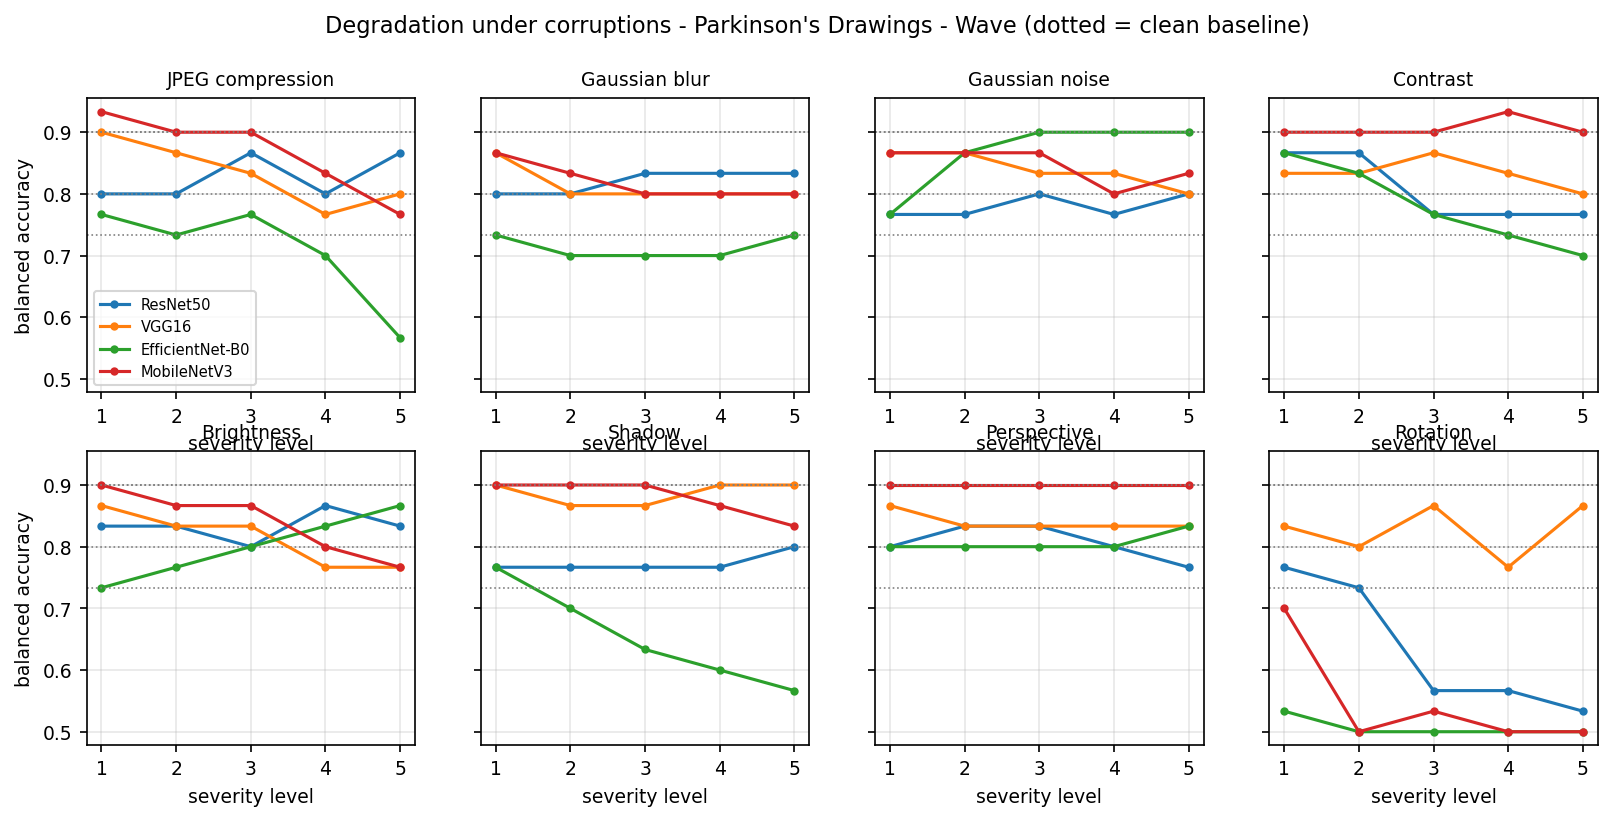
\includegraphics[width=0.98\linewidth]{figures/fig_curves_pdraw_wave.png}
\caption{PDRAW--wave.}
\end{figure}

\begin{figure}[h]
\centering\small
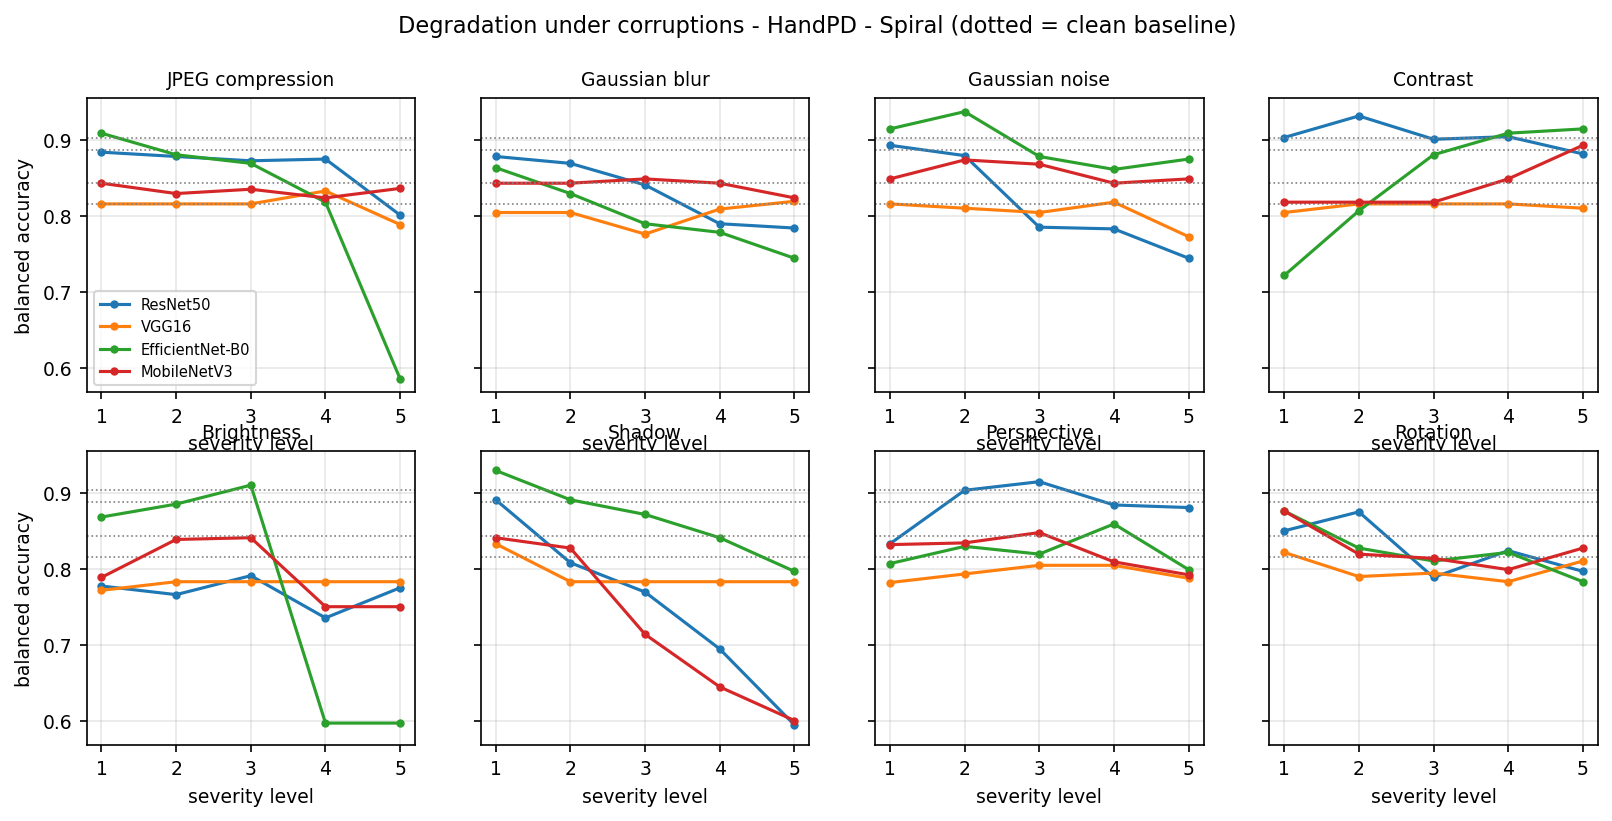
\includegraphics[width=0.98\linewidth]{figures/fig_curves_handpd_spiral.png}
\caption{HandPD--spiral.}
\end{figure}

\begin{figure}[h]
\centering\small
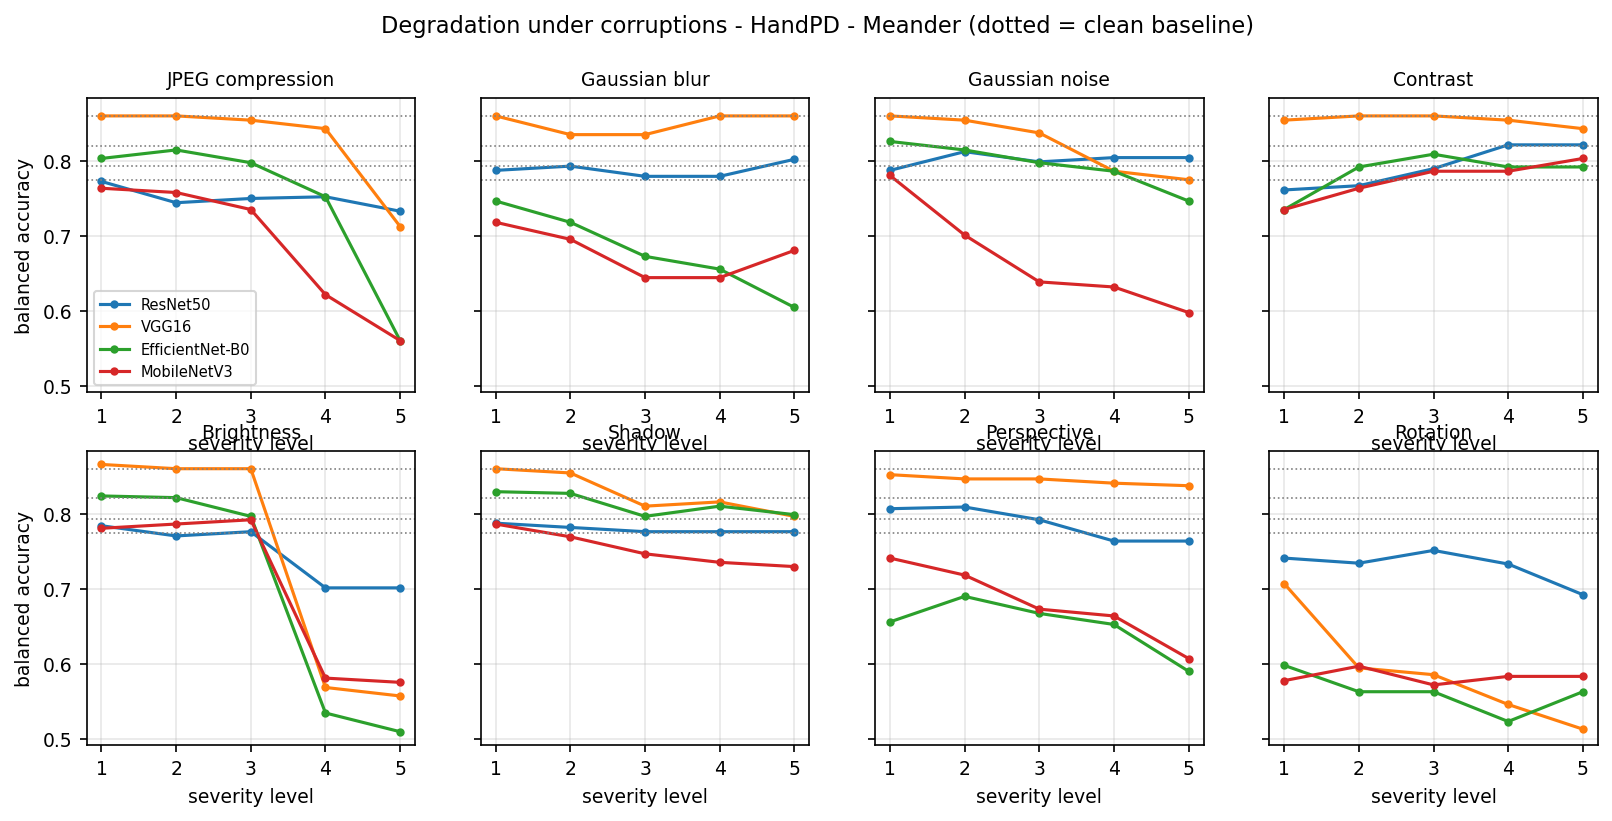
\includegraphics[width=0.98\linewidth]{figures/fig_curves_handpd_meander.png}
\caption{HandPD--meander.}
\end{figure}

\section*{S5. Grad-CAM randomization control}
As reported in Section~5.3 of the main text, replacing the trained head and
fine-tuned last stage with freshly initialized parameters collapses the rank
agreement with the trained models' clean Grad-CAM maps (mean Spearman on the
PDRAW--spiral subset: ResNet50 0.23, VGG16 $-0.15$, EfficientNet-B0 0.04,
where the untrained EfficientNet produces constant maps). Per-image values
are released as \texttt{results/gradcam\_sanity.csv}. This control supports
that the measured corruption effects (Section~5) reflect model-specific
learned evidence rather than input-only structure, while leaving the
stability-versus-validity distinction of the main text unchanged.

\end{document}
